% !TeX root = ../thuthesis-example.tex

\chapter{集群故障检测和判断}

集群故障检测和判断是构建高可用自动容错能力的先决条件。如同医生诊断病情是进行治疗的第一步,系统也必须先感知到问题的存在,才能采取相应的应对措施。及时、准确地识别出集群中发生的各种故障,是后续所有容错机制得以有效运行的前提。

本章节描述了高可用框架下的集群故障检测和判断机制。ConfigNode是集群的大脑,负责集群故障检测和研判。ConfigNode通过和集群所有成员交换心跳定期收集信息,并使用集群故障研判的算法来发现故障。

本节描述了ConfigNode和DataNode之间、DataNode和DataNode之间的定期心跳交换机制,以及在心跳中交换节点基本信息、负载状况、网络拓扑的方法。
同时,本节描述了基于心跳历史的Phi Accrual研判算法,使用收集到的心跳内容进行故障的概率判断。最后,本节描述了基于Thrift的快速故障研判的优化。

\section{ConfigNode和DataNode的心跳机制}

IoTDB通过ConfigNode和DataNode定期交换心跳的机制来维护每一个DataNode节点的信息,并用这些信息进行磁盘、进程和对称网络分区的故障探测。本节阐述了ConfigNode和DataNode之间心跳交换的具体实现。

ConfigNode会将集群的所有节点纳入心跳管理的范畴。具体来说,无论是ConfigNode、DataNode还是AINode,在启动时都需要向ConfigNode的Leader节点汇报和注册自己。一经注册,ConfigNode Leader就会将这个进程纳入到心跳管理的范围内。同样,在节点下线维护、被移出集群、重启时也会向ConfigNode进行汇报,由ConfigNode决定是否要将节点移除出心跳管理的范畴。

对于纳入心跳管理范畴的节点,ConfigNode会按照固定时间间隔(默认为1s)向这些节点的内部端口发送RPC心跳探测,并要求节点上传自身的信息,确认最新的状态。以DataNode为例,DataNode需要通过心跳上报当前的存活状态、节点的CPU负载率、内存占用率、磁盘的消耗情况以及DataNode上每一个Region的情况,包括Region Leader的身份确认、每一个Region的磁盘占用情况、副本日志同步的情况、DataNode上所有pipe任务的情况。

通过定期交换信息,ConfigNode能够掌握节点的全局信息,并利用上述这些信息展开对磁盘写满、节点宕机、网络对称分区等错误的检测。具体的检测方法可以参考后续的章节\ref{failure_detection}。

\section{DataNode和DataNode的心跳机制}


通过ConfigNode和DataNode的心跳,IoTDB已经能够有效地检测每个节点的存活状态。
然而,这个心跳机制在面对DataNode之间非对称网络分区这种复杂且隐蔽的场景时,却无法进行准确的检测。

\subsection{非对称网络分区问题描述}
非对称网络分区 (Asymmetric Network Partition)指的是某些DataNode节点能够向其他节点发送消息,但是无法接收来自这些节点的消息,或者反过来,接收消息正常但发送消息受阻。这种单向或双向但方向不同的通信故障,与传统的对称网络分区(即一组节点完全无法与另一组节点通信)有着本质的区别。严格来讲,现有的ConfigNode和DataNode之间的心跳只能验证两个节点之间的双向通信的有效性,但无法验证DataNode和DataNode之间的通信的有效性。

\begin{figure}
  \centering
  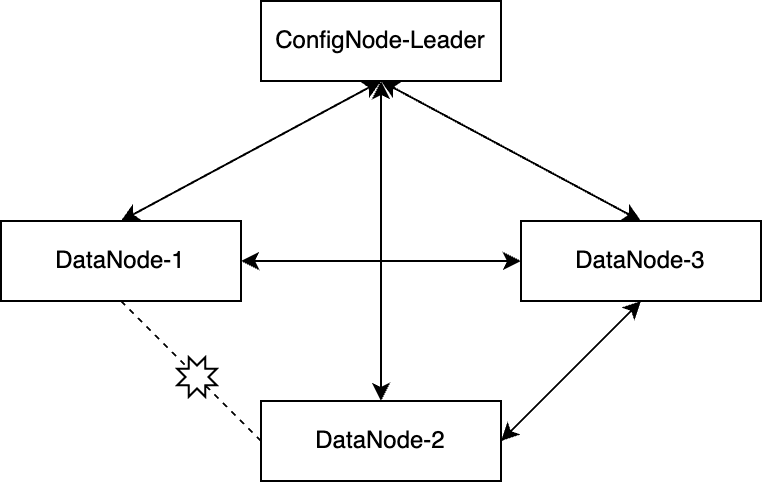
\includegraphics[width=0.9\linewidth]{c03-parition.png}
  \caption{系统非对称分区示意图}
  \label{fig:c03-partition}
\end{figure}

考虑图\ref{fig:c03-partition}所示的系统情况,集群由1个ConfigNode和3个DataNode组成,其中ConfigNode和所有三个DataNode都能正常连接交换情况,但是DataNode1和DataNode2之间的网络连接可能因为配置不当或者线缆断裂而出现非对称网络分区。这种非对称网络分区的问题不能被上述提到的心跳机制所捕捉。这种未被检测到的非对称网络分区会极大地影响系统的可用性,可能造成的问题包括但不限于:

1. 影响共识模块的可用性保证。在RatisConsensus中,如果是两副本,并且两个副本分别处在非对称分区的两个节点DataNode1和DataNode2上,那么这个共识组在事实情况下处在不可用状态,需要进行相关的恢复策略。

2. 影响DataNode对客户端提供的服务保证。如果客户端需要将数据写入集群,且副本位于DataNode2上,那么客户端只能连接DataNode2直接写入或者通过DataNode3进行转发。如果客户端连接DataNode1,那么这次写入会在超时后失败,影响系统的高可用性保障。

3. 影响集群的查询能力。集群在查询调度的规划时,如果对网络可达性不了解,那么查询计划可能会错误的生成,导致这个查询计划最终失败。在章节\ref{sec:topology-query-plan}中对这一部分的错误有详细的说明。

\subsection{DataNode间的对等心跳}\label{sec:datanode-intra-heartbeat}

为解决上述的非对称网络分区的检测的问题,本文提出基于DataNode间的对等心跳汇总的集群拓扑感知机制,通过DataNode之间定期交换心跳来获取相互之间的连通性,并将所有节点的结果汇总上报给ConfigNode Leader,从而使ConfigNode Leader具备集群的网络拓扑感知能力。

\begin{figure}
  \centering
  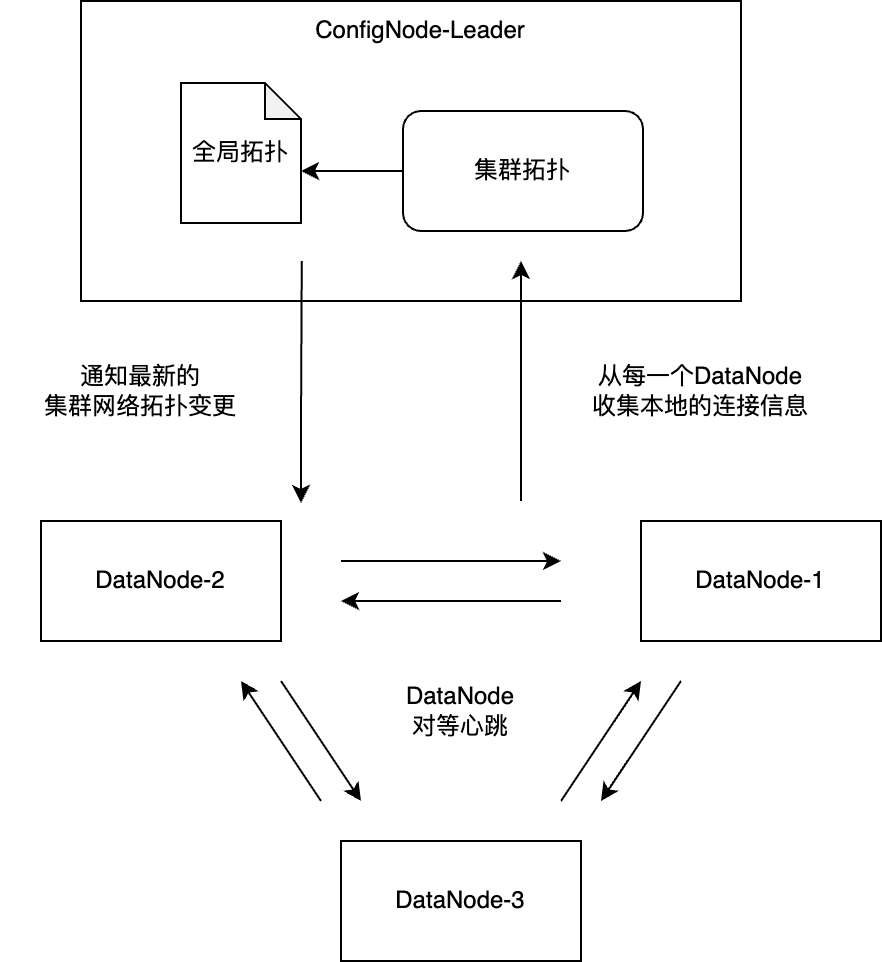
\includegraphics[width=0.7\linewidth]{c03-topology-redraw.png}
  \caption{集群拓扑感知能力}
  \label{fig:c03-topology}
\end{figure}

图\ref{fig:c03-topology}给出了DataNode间的对等心跳机制描述。

ConfigNode会定期要求集群中的每个 DataNode 都与其他 DataNode 进行对等的心跳交换。通过这种全互联的心跳机制,每个 DataNode 能够更直接地获取自己与其他 DataNode 之间的网络连通性状态,例如是否能够成功发送心跳、是否能够及时收到对方的心跳响应等。

随后,每个 DataNode 会将自己收集到的与其他 DataNode 的连通性信息进行汇总和整理,形成一个局部的网络拓扑视图。这个视图包含了该 DataNode 对集群中其他 DataNode 可达性的判断。

为了获得全局的视角,每个 DataNode 会将这个汇总后的连通性报告定期地上报给当前激活的 ConfigNode Leader。ConfigNode Leader 作为集群的中央协调者,在接收到来自所有 DataNode 的连通性报告后,便能够汇总所有节点的局部视图,从而构建出一个完整的、全局的集群网络拓扑感知能力。与仅仅依赖 ConfigNode 和 DataNode 之间的单向心跳相比,这种方式能够更全面地了解集群内部节点之间的双向通信状况。

在获取了全局视角的网络拓扑图之后,ConfigNode会通过RPC的方式将这个全局拓扑下放通知给所有的DataNode,从而赋予每一个DataNode更加完善的集群状态感知能力,允许在后续的写入规划、查询规划等操作更加智能、可靠。


\section{基于Phi Accrual算法的故障研判}\label{failure_detection}

\subsection{基于心跳固定超时时间的判断}\label{failure_detection_timeout_fix}

在本文的工作之前,IoTDB内部采用基于心跳固定超时时间的故障检测。该算法可以概括为,如果节点在超过一段时间之后没有收到另外一个节点的心跳,那么就会认为另外的这个节点出现了故障,可能是网络分区或者进程宕机。
更具体地,我们定义超时时间参数$\Delta_{t}$(默认为20s),该参数的含义是:当ConfigNode Leader在超过$\Delta_{t}$的时间里面没有收到某一个被询问方DataNode的心跳,或者发起方DataNode在超过$\Delta_{t}$的时间里没有收到另外的一个被询问方DataNode的心跳,就会判断被询问方的DataNode不可达,可能是出现了网络分区或者其他问题。

这种基于心跳的固定超时算法的优点在于逻辑简单直接,易于实现和部署,并且在IoTDB已有的实践中能胜任大部分的错误发现。然而这种算法依然存在诸多问题,例如:

1. 固定的算法无法应对复杂和变化的系统环境。节点的网络变化、系统的负载变化、长时间的GC等诸多因素都有可能导致心跳包被延迟传输或拥塞,从而出现超时产生误判,触发不必要的容错操作。

2. 选择一个$\Delta_{t}$ 的最佳参数在实践中非常困难。一方面,参数的选择需要人工介入,需要用户对自身业务集群的特性、IoTDB内核的故障检测机制都有所了解,这对很多用户来说是一个很大的心智负担。
另一方面,参数 $\Delta_{t}$ 本身就是故障检测的检测速度和检测正确度的权衡。选择一个较短的$\Delta_{t}$参数,那么节点故障会被快速发现,但对应的误报率就会很高;如果选择一个较长的$\Delta_{t}$,虽然误报率会对应下降,但是错误的平均发现时间将会变长。

\subsection{IoTDB故障研判算法}

章节\ref{sec:cassandra-failure-detecttion}提到的Phi Accrual能够良好解决上述的两个问题。然而,Phi Accrual算法存在冷启动的问题。在节点启动、重启的阶段,如果错误地将节点判断成不可达,那么可能会导致不必要的故障转移、节点延迟加入集群或提供服务和增加运维复杂性等问题。

为此,本文最后提出的IoTDB故障研判算法是结合心跳固定超时时间的判断和Phi Accrual算法的结果。具体来说,IoTDB的故障检测将会根据节点的生命周期划分为两个阶段:冷启动阶段和正常服务阶段。

冷启动阶段。当节点刚刚启动,或是刚刚从故障恢复,此时我们尚未收集到足够的心跳样本,我们将会使用\ref{failure_detection_timeout_fix}提到的算法来负责初始时期的节点故障检测,并同时在后台继续收集样本。当我们收集了足够的样本数量(默认为60个)的时候,我们切换成基于Phi Accrual的算法来研判节点的存活率。由于节点在刚启动过程中往往不会立马承担较大的流量负载,也不太可能会发生长时间的垃圾回收等异常情况,因此在这个阶段使用固定超时算法将能较为有效地实现故障检测。

节点正常服务阶段。当节点稳定提供服务一段时间之后,我们已经收集到了足够的心跳历史样本,IoTDB集群将会切换为基于Phi Accrual的检测算法进行故障研判。具体的实现如下:

1. 收集心跳历史采样。对于每一个新到达的心跳包,算法会计算出和上一个心跳包之间的间隔,并将这个间隔存入一个固定大小(默认为100)的采样窗口内。当有新的心跳不断到达的时候,最新的一个间隔会被存入采样窗口,窗口最早的第一个间隔则会被剔除,以便更好地反映集群的近况。

2. 根据采样窗口计算到达间隔的分布,计算 $\phi$ 值。在Phi Accrual算法中, $\phi$ 值代表了一个节点出现故障的怀疑概率。
我们假设心跳到达间隔的分布符合正态分布,那么可以通过历史采样窗口来估计分布的均值 $\mu$ 和方差 $\sigma^2$。那么,在上一次心跳到达t时间之后才会有下一次心跳到达的概率可以通过下列公式计算出来:


$$ P_{later}(t) = \frac{1}{\sigma\sqrt{2\pi}} \int_{t}^{\infty} e^{-\frac{(x-u)^2}{2\sigma^2}} dx $$

在实际实现中,我们通过逻辑斯蒂分布对高斯分布进行近似\cite{bronvstejn2013handbook}:

$$ P_{later}(t) = \exp(1.5976 + 0.070566 (\frac{t-u}{\sigma})^2) $$


3. 计算 $\phi$ 并根据设定阈值进行比较。我们使用如下的公式进行定义:

$$ \phi(now) = -log_{10}(P_{later}(t_{now} - t_{last})) $$

用户可以通过设定不同的$\phi$阈值来控制研判的精准度。阈值越高,研判的精准度越高。在章节\ref{exp-phi}中,我们给出了这个故障检测算法的实验验证和不同阈值参数下算法的表现行为。


\section{基于集群可观测性的故障发现}

在上述的内容中,我们探讨了IoTDB中基于心跳机制的节点的自动故障发现。本节将会简单介绍如何利用集群的可观测性,并结合人为参与,来更全面地发现和诊断集群中潜在的或已发生的故障。

\subsection{可观测性的建设}

可观测性是指系统通过其外部输出(如指标、日志和追踪)来推断其内部状态的能力。在故障发现的场景下,可观测性扮演着至关重要的角色,它能够帮助我们发现自动化系统未能识别的异常、在发生故障之后理解故障的根本原因。

IoTDB内部构建了基于指标 (Metrics)、日志 (Logs)、追踪 (Traces)三位一体的可观测性系统。以监控为例,IoTDB构建了系统资源监控和功能模块监控。
系统资源的监控包括了CPU、磁盘、网络、JVM线程、内存使用情况、垃圾回收状况等。
功能模块的监控包括了存储引擎、元数据管理引擎、查询引擎、共识模块和Pipe模块内部定义的相关指标。

\subsection{基于可观测性的故障优化}

在可观测性的基础上,我们可以进一步完善故障的发现和分析和改进流程。
目前,IoTDB的可观测性会参与到故障发生的前中后全生命周期中,用例包括但不限于:

1. 故障发生前的告警。运维和测试人员可以通过针对关键指标(如错误率、请求延迟、资源使用率)预先设定阈值,由可观测性平台在指标超出正常范围时发出告警。后续,也可以通过自动的算法对关键指标的历史数据进行趋势分析,识别出异常的前兆,在故障真正影响用户之前防患于未然。

2. 故障发生时的快速定位。在错误发生时,相关开发人员或运维人员可以通过监控面板的各个仪表盘、实时的错误日志和堆栈信息进行分析,更加快速地定位错误的节点、进程、模块,速缩小故障排查范围,提高诊断效率。

3. 故障发生后的改进和优化。IoTDB的开发人员可以通过历史可观测数据,在日常开发或者故障发生之后,更好地理解系统行为,深入分析集群的性能、资源利用率、功能是否达到预期,从而对系统进行更精准的改进,提升开发团队的工作效率。


\section{基于Thrift长连接的进程失效快速检测优化}\label{sec:detection-thrift}

在\ref{failure_detection}中提到的故障研判,通过对心跳行为建立概率模型来判断节点是否发生故障。这种故障研判需要一定的观察窗口才能作出可靠的判断,因此发现故障通常需要十秒或者更久。

然而,在进程宕机、被系统强制关闭等特殊场景下,我们可以利用Thrift 长连接的特点,将被动的故障发现转化为主动的故障通知,从而显著加快故障的发现和传播速度。

IoTDB内部采用Thrift\cite{slee2007thrift}框架作为RPC通信的实现。Thrift框架底层使用网络协议层的TCP协议或者UDP协议实现实际的传输。IoTDB 内部采用 ClientManager 接口来统一管理对外的 Thrift 连接。ClientManager 的基本原理类似于带缓存的连接池。当我们首次请求连接到某一个新的 EndPoint(代表一个特定的 IP 地址和端口)时,ClientManager 会建立一个底层的 TCP 连接。与使用完毕后立即断开连接不同,ClientManager 会在结束使用后继续维持这个 TCP 连接一段时间,并将其缓存在本地。这样,在下次我们需要请求相同的 EndPoint 地址时,就不需要重新进行 TCP 三次握手等连接建立的开销,可以直接复用 ClientManager 内部缓存的现有连接。只有当某个 TCP 连接长时间没有被使用时,ClientManager 才会主动销毁该连接并清理相关的系统资源。

由于 ConfigNode 和每一个 DataNode 之间存在持续频繁的内部 RPC 通信,通过上述所言的 ClientManager 的机制,我们可以认为在 ConfigNode 和 DataNode 之间建立了一条长期有效的 TCP 连接信道,并在这个 TCP 信道的基础上建立了一个长期有效的 Thrift 连接。

Thrift框架能够感知其底层的TCP传输层的连接状态。当连接的进程突然出现故障,无论是是由于程序崩溃,还是被操作系统强制终止(例如使用 kill -9 命令),该进程所建立的TCP连接也会中断。
Thrift 能够迅速检测到这个信道的问题,并向上层的IoTDB模块汇报连接中断的事件。
这种主动汇报机制的时间延迟通常在故障发生的毫秒到秒级,非常快速。

ConfigNode Leader会利用这样的机制,在收到断开汇报的时候将该进程标记为失效,从而实现进程失效的快速检测和优化。